% !TeX document-id = {5986425d-2453-4c25-8285-071593d24d0f}
% !TeX TXS-program:compile = txs:///pdflatex/[--shell-escape]
\documentclass{article}

\usepackage[utf8]{inputenc}
\usepackage[T1]{fontenc}
\usepackage{color}
\usepackage{soul}
\usepackage{amsmath}
\usepackage{amssymb}
\usepackage{listings}
\usepackage{minted}
\usepackage{hyperref}
\usepackage{graphicx}
\usepackage{calc}
\usepackage{enumitem}
\usepackage{standalone}

\graphicspath{{img/}}
\setlength{\parindent}{0pt}

\begin{document}

\section{USRP Hardware Problems} 

\subsection{How It Is Supposed to Work}

The following plots show the output of a successful measurement with two USRPs using CSMA/CA, although measurement 4 is a little bit messed up as well. Note that wrong x-axis on the line chart has been fixed by the time writing this.

\bigskip

\textbf{Note:} Always take a look at the y-axis scaling. While such data representation might confuse the skimming reader it allows for higher resolution. Also note that not every plot adds more information, this also has the purpose of showcasing different plot types. And as a FYI: the linear interpolation in the line chart can be replaced with any other form of interpolation making it potentially more informative than the bar chart.

\begin{figure}[h] \label{usrp-success-1}
	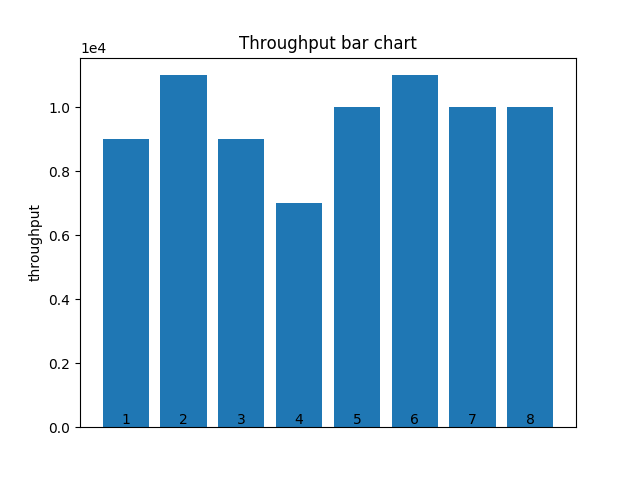
\includegraphics[width=\textwidth]{usrp_success_tp_bar}	
\end{figure}

\begin{figure}[ht] \label{usrp-success-2}
	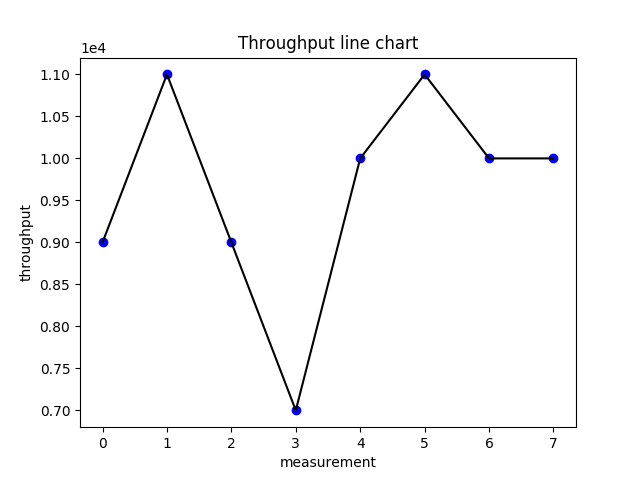
\includegraphics[width=\textwidth]{usrp_success_tp_line}	
\end{figure}

\begin{figure}[h] \label{usrp-success-3}
	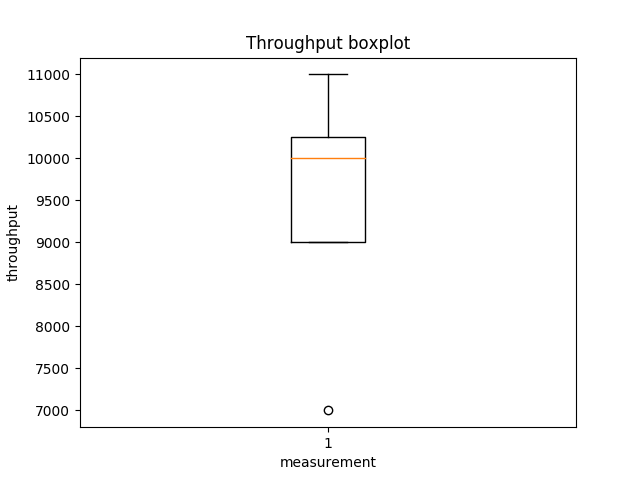
\includegraphics[width=\textwidth]{usrp_success_tp_boxplot}	
\end{figure}

\begin{figure}[h] \label{usrp-success-4}
	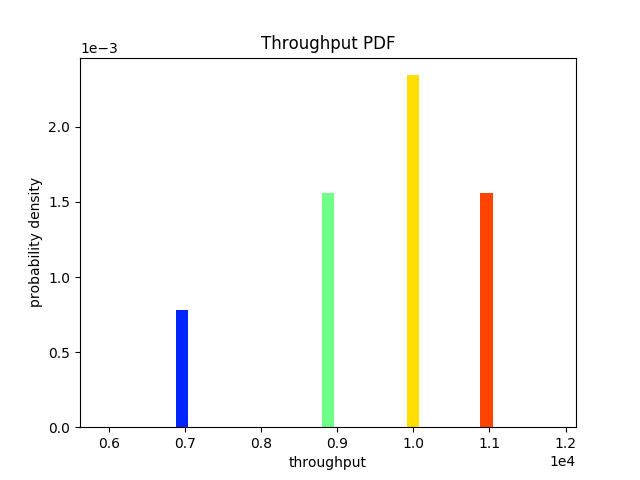
\includegraphics[width=\textwidth]{usrp_success_tp_pdf}	
\end{figure}

\begin{figure}[h] \label{usrp-success-5}
	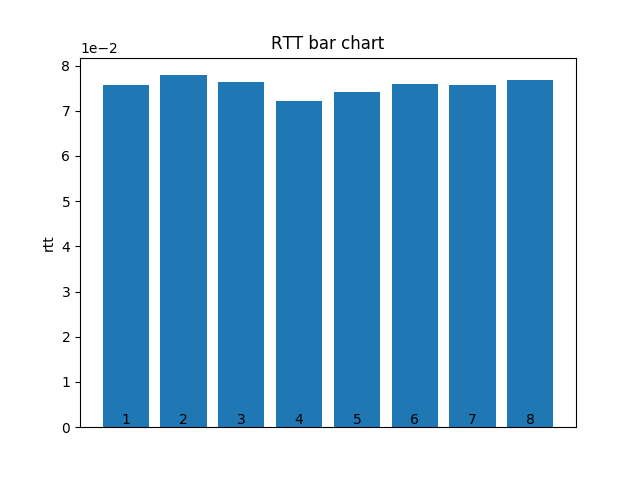
\includegraphics[width=\textwidth]{usrp_success_rtt_bar}	
\end{figure}

\begin{figure}[h] \label{usrp-success-6}
	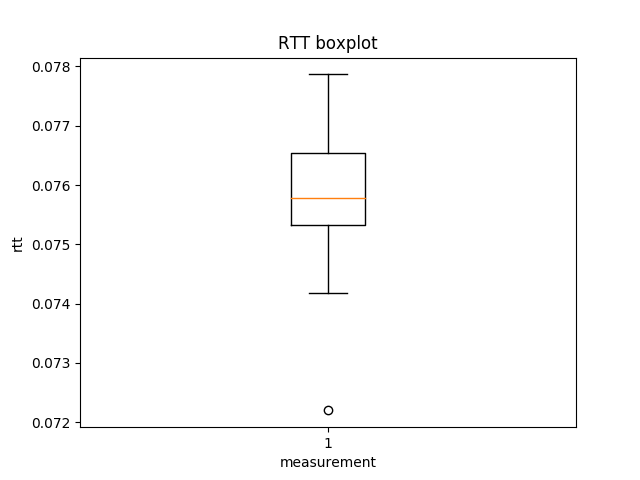
\includegraphics[width=\textwidth]{usrp_success_rtt_boxplot}	
\end{figure}

\begin{figure}[h] \label{usrp-success-7}
	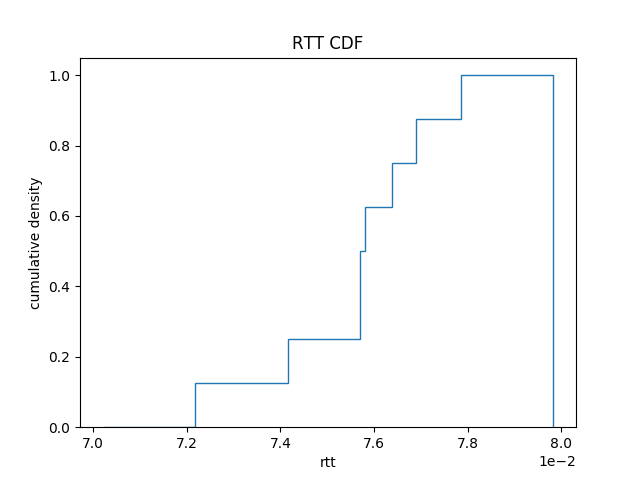
\includegraphics[width=\textwidth]{usrp_success_rtt_cdf}	
\end{figure}

\clearpage

\subsection{Failure Pattern 1}

The following six figures visualize an issue I'm experiencing with the USRPs whose origin I have difficulties to track down. In seemingly random patterns the devices fail for the rest of the transmission. To make matters worse, it is not obvious whether the problem is enitrely hardware-related or has some software-related component. Let me first explain what happens in the following plots, though.

\bigskip

In the throughput bar chart it is obvious the device failed during the measurements 2 and 20. The logs of the measurement and this suggest that this could very well be a software problem.
After 17 seconds the sender doesn't send any frames anymore (frame\_probe 850 is not reached anymore). Once the sender fails it doesn't recover until the measurement script and the next measurement is launched, which is a reason to suspect a software failure on either my side or Gnu Radio's. 

\bigskip

Note that the obviously wrong RTT in measurement 18 is due to the fact that retransmissions are
taken into account when calculating the RTT. A fix for that is yet to  be found. Alternatively, or as an alternative mode taking retransmissions into account with retransmission counters to calculate the frame delay instead of the RTT is being considered. However, at the moment there exist practical implementation barriers that are to be removed.

\begin{figure}[h] \label{usrp-fails-4}
	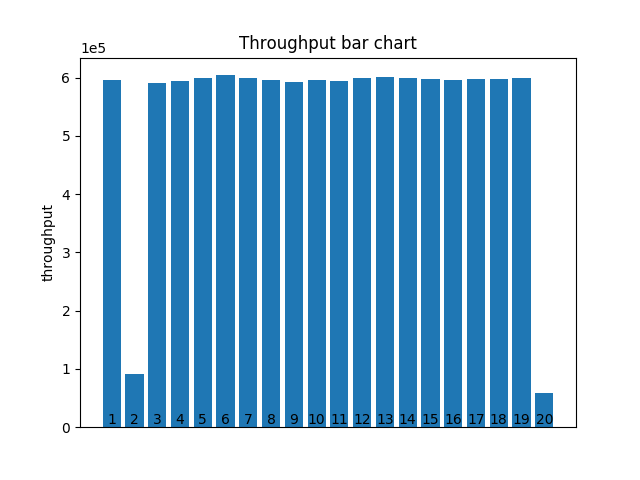
\includegraphics[width=\textwidth]{usrp_fail_tp_bar}	
\end{figure}

\begin{minted}[tabsize=4]{bash}
### This is from the measurements logs
Measurement 2/20 complete in 100 second(s).
# ... cut ...
Measurement 2/20 complete in 83 second(s).
++++ frame_probe ID: 860 receives a frame at time 71.8424s ++++
++++ frame_probe ID: 1010 receives a frame at time 71.846s ++++
++++ frame_probe ID: 890 receives a frame at time 71.8708s ++++
the 100th message counter  has been visited 89 times  
++++ frame_probe ID: 850 receives a frame at time 71.9534s ++++
INFO: Detected an invalid packet at item 8544
INFO: Parser returned #f
++++ frame_probe ID: 860 receives a frame at time 71.9941s ++++
++++ frame_probe ID: 1010 receives a frame at time 71.9994s ++++
++++ frame_probe ID: 890 receives a frame at time 72.0241s ++++
the 100th message counter  has been visited 90 times  
++++ frame_probe ID: 850 receives a frame at time 72.0925s ++++
INFO: Detected an invalid packet at item 8640
INFO: Parser returned #f
++++ frame_probe ID: 860 receives a frame at time 72.1332s ++++
++++ frame_probe ID: 1010 receives a frame at time 72.1437s ++++
++++ frame_probe ID: 890 receives a frame at time 72.1685s ++++
the 100th message counter  has been visited 91 times  
Measurement 2/20 complete in 82 second(s).
Measurement 2/20 complete in 81 second(s).
Measurement 2/20 complete in 80 second(s).
Measurement 2/20 complete in 79 second(s).
Measurement 2/20 complete in 78 second(s).
Measurement 2/20 complete in 77 second(s).
Measurement 2/20 complete in 76 second(s).
Measurement 2/20 complete in 75 second(s).
Measurement 2/20 complete in 74 second(s).
Measurement 2/20 complete in 73 second(s).
Measurement 2/20 complete in 72 second(s).
# ... cut ...
Measurement 2/20 complete in 2 second(s).
Measurement 2/20 complete in 1 second(s).
\end{minted}

\begin{figure}[h] \label{usrp-fails-5}
	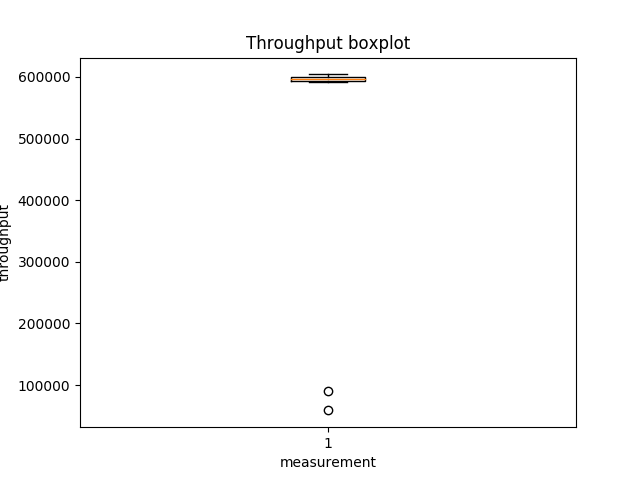
\includegraphics[width=\textwidth]{usrp_fail_tp_boxplot}
	
\end{figure}

\begin{figure}[h] \label{usrp-fails-6}
	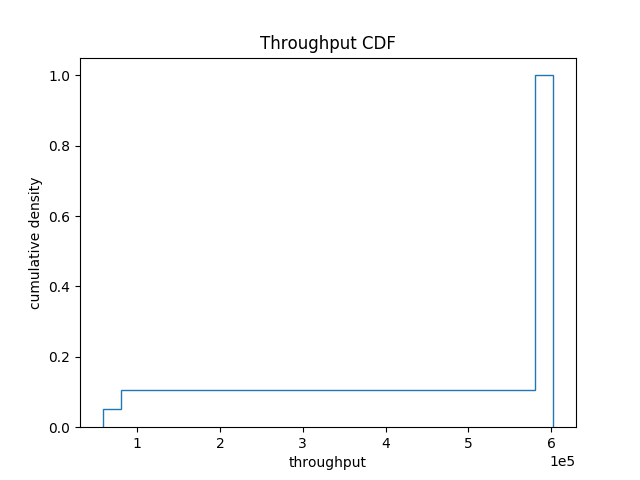
\includegraphics[width=\textwidth]{usrp_fail_tp_cdf}	
\end{figure} 

\begin{figure}[h] \label{usrp-fails-1}
	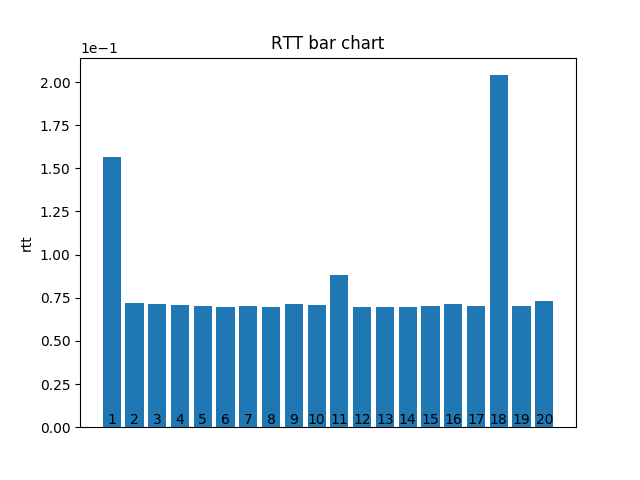
\includegraphics[width=\textwidth]{usrp_fail_rtt_bar}
	
\end{figure} 

\begin{figure}[h] \label{usrp-fails-2}
	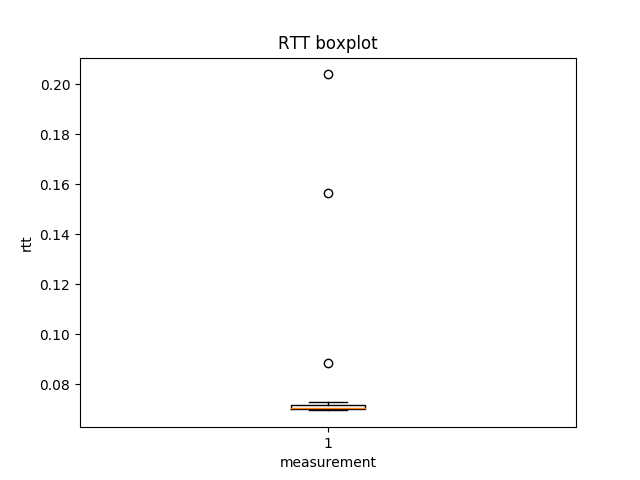
\includegraphics[width=\textwidth]{usrp_fail_rtt_boxplot}
\end{figure}

\begin{figure}[h] \label{usrp-fails-3}
	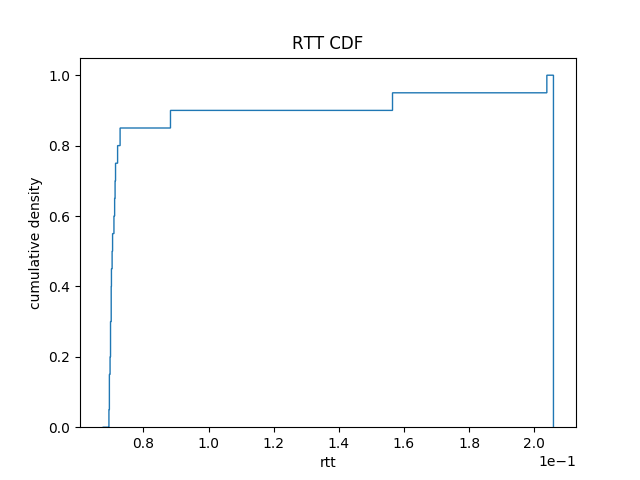
\includegraphics[width=\textwidth]{usrp_fail_rtt_cdf}
\end{figure}

\clearpage

\subsection{Failure Pattern 2}

However, the failures are not permanent and show no repetitive pattern. Furthermore, during the problematic sections \texttt{uhd\_find\_devices} does not detect any USRPs anymore. From these two facts one can deduce the problem at least has a hardware component. Here are some plots of a typical measurement with hardware failure. 

\bigskip

Although for 7 out of 10 measurements the throughput \text{seems} - i.e. it is NOT - reasonable a lot of ACKs got lost during the transmission. Note that due to the problem described in the previous section the RTT calculation is wrong, because lost ACKS affect the RTT value for all following data transmissions (continuous additive error on fail). The throughput is reduced by a factor 6 for unknown reasons. Compare this to the last section if you want to see what I mean (both measurements had single submeasurement durations of 100s).

\bigskip

Proof for lost ACKs can be found as mentioned in the RTT charts as well as in the logs. Note that the setup and parameters including receive and transmission gains were chosen no different from those in the previous section, which is a strong indication of either hardware failure or external influence which in should have been covered by choosing an unused sending frequency. 

\begin{figure}[h] \label{usrp-fails2-1}
	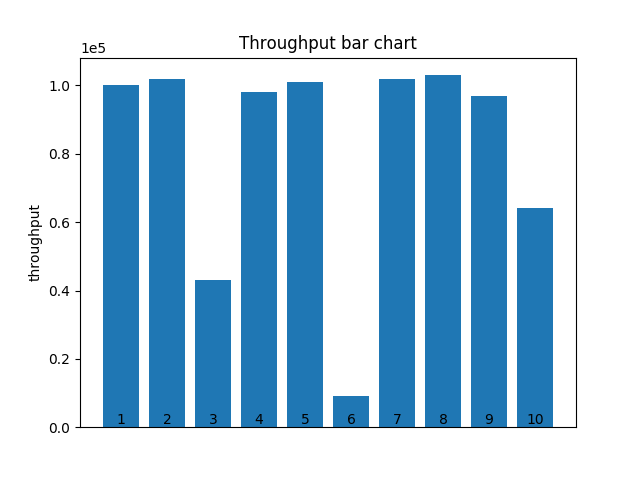
\includegraphics[width=\textwidth]{usrp_fail2_tp_bar}
	
\end{figure}

\begin{figure}[h] \label{usrp-fails2-2}
	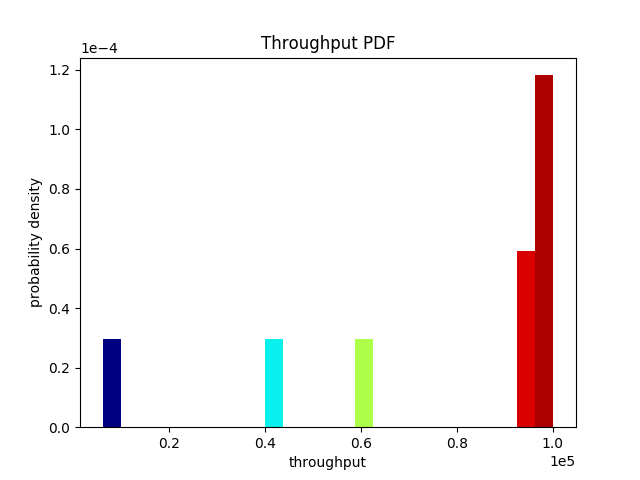
\includegraphics[width=\textwidth]{usrp_fail2_tp_pdf}	
\end{figure} 

\begin{figure}[h] \label{usrp-fails2-3}
	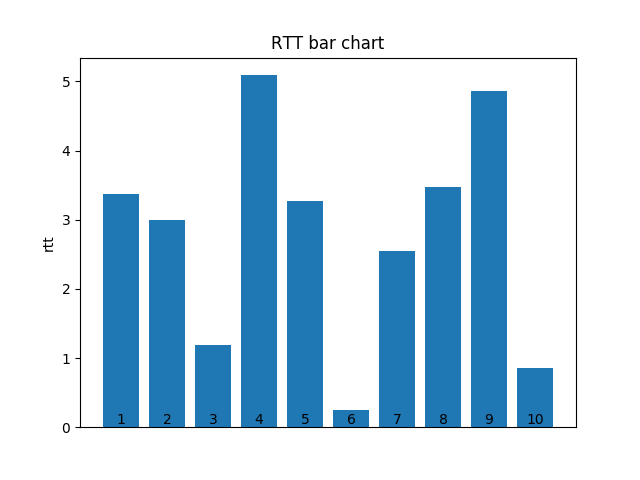
\includegraphics[width=\textwidth]{usrp_fail2_rtt_bar}
	
\end{figure} 

\begin{figure}[h] \label{usrp-fails2-5}
	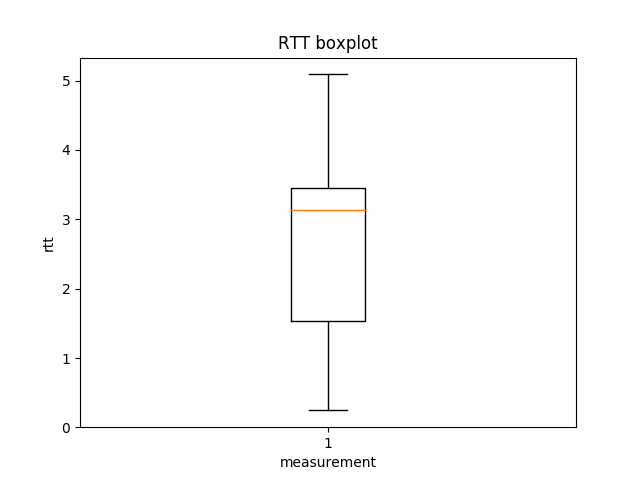
\includegraphics[width=\textwidth]{usrp_fail2_rtt_boxplot}
\end{figure} 

\clearpage

\subsection{Justification of Measurement Results}

\subsubsection{RTT}

The following section is concerns the CSMA/CA two-way handshake (no CTS/RTS).

In the "flawless" measurement plots both the RTT and the throughput don't differ significantly from the theoretical calculation following:

Theoretical:
\begin{equation*}
\begin{split}
	RTT & = 2 \cdot t_{prop}+t_{data}+t_{ack}+2\cdot t_{proc}+\text{DIFS}+\text{SIFS} \\
		& = \delta_{prop}+0.04s+t_{ack}+2t_{proc}+0.018s+0.006s \\
		& = 0.064s + \delta_{prop} + t_{proc} +t_{ack}
\end{split}
\end{equation*} 

Where $\delta_{prop} \approx 10^{-10}s \approx 0 $

\bigskip

Measured:~0.075s 

\subsubsection{Throughput}

\bigskip

Theoretical (assuming RTT is correctly determined):
\begin{equation*}
\begin{split}
	\text{throughput} & = \frac{s_{frame}}{t_{frame}} = \frac{\text{packet size}}{\text{RTT}} \\
	& \approx \frac{1000B}{0.075s} \\
	& \approx 13333B/s
\end{split}
\end{equation*}

So for a 100s measurement the theoretical throughput should be roughly $1.3\cdot 10^6$.

Measured: $6 \cdot 10^5$

\bigskip

The RTT measurements can be further backed up by measuring the RTT with linear increasing SIFS. The expected RTT then would be a linear function of SIFS.

\bigskip

Analogously, throughput should be a linear function of packet size. 

\bigskip

Note that for both such measurements a sufficiently large measurement time must be chosen to counteract various random influences.

\subsubsection{Retransmissions}
Result can be roughly verified by comparing throughput versus theoretical throughput (channel busy time not taken into account with only one pair of sender and transmitter). For a multiple sender scenario one has to take backoff times into account as well.

\end{document}